\documentclass[11pt]{article}
\usepackage{calc}
\usepackage[margin={1in,0.5in},footskip=0in]{geometry}
\usepackage[miniquiz]{hwk}
\usepackage{tikz}

\renewcommand{\theclass}{math 1300}
\renewcommand{\dateinfo}{September 11, 2012}
\renewcommand{\theassignment}{Quiz 2}

\begin{document}
\pagestyle{empty}
\newsavebox{\quizfront}
\begin{lrbox}{\quizfront}
\begin{minipage}[top][4.5in][t]{\textwidth} \setlength{\parindent}{1.5em}
\drawtitle
\vspace{-0.5in}
\begin{enumerate}

\item The graph of $y=f(x)$ is shown.  Sketch the graph of
  $y=f^{-1}(x)$ on the same axes.

\vfill

  \begin{center}
    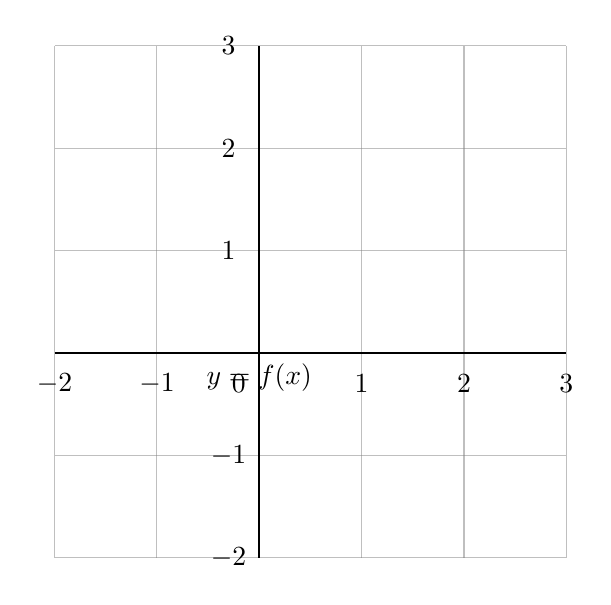
\begin{tikzpicture}[scale = 1.3]
      \def\xmin{-2}\def\xmax{3} \def\ymin{-2}\def\ymax{3} 
      \foreach \i in {\xmin,...,\xmax} {\ifnum\i=0{}
        \else{\draw[gray, thin, opacity=.5]
          (\i,\ymin) -- (\i,\ymax);\draw node at (\i, -.3) {$\i$};}\fi}
      \foreach \i in {\ymin,...,\ymax} {\ifnum\i=0{}
        \else{\draw[gray, thin, opacity=.5]
          (\xmin, \i) -- (\xmax, \i);\draw node at (-.3, \i) {$\i$};}\fi}
      \draw node at (-.2, -.3) {$0$};
      
      \draw[thick] (\xmin,0) -- (\xmax,0); \draw[thick] (0,\ymin) --
      (0,\ymax);
      
      \draw[very thick, domain=-2:\xmax, -] plot[samples=200]
      function{((x-1)/abs(x-1))*abs(x-1)**(1.0/3)+1} node[below]{$y=f(x)$};
    \end{tikzpicture}

  \end{center}

  \vfill

\end{enumerate}
\begin{flushright}
Problem on the back $\longrightarrow$
\end{flushright}



\end{minipage}
\end{lrbox}

%%%%%%%%%%%%%%%%%%%%%%%%%%%%%%%%%%%%%%%%%%%%%%%%%%%%%%
%%%% This is for the back of the quiz
%%%%%%%%%%%%%%%%%%%%%%%%%%%%%%%%%%%%%%%%%%%%%%%%%%%%%%
\newsavebox{\quizback}
\begin{lrbox}{\quizback}
\begin{minipage}[top][4.5in][t]{\textwidth} \setlength{\parindent}{1.5em}
\begin{itemize}
\item[2.] Solve the following equation for $x$:
  \[
  3^x = 5\cdot 2^x.
  \]


\end{itemize}
\end{minipage}
\end{lrbox}

%%%%%%%%%%%%%%%%%%%%%%%%%%%%%%%%%%%%%%%%%%%%%%%%%%%%%%
%%%%
%%%% Now we make two copies of the ``quizfront'' box
%%%%
%%%%%%%%%%%%%%%%%%%%%%%%%%%%%%%%%%%%%%%%%%%%%%%%%%%%%%%
\noindent \usebox{\quizfront}
\vfill
\noindent \usebox{\quizfront}

%%%% Uncomment the rest to have a two-sided quiz.
\pagebreak
\noindent \usebox{\quizback}
\vfill
\noindent \usebox{\quizback}
\end{document}